\chapter{Fonctions analytiques}
\section{Rappels sur les nombres complexes}
  %  \textit{Les pré-requis du cours de Connaissances Fondamentales concernant les nombres
   % complexes sont disponibles en Annexe A.}
    \subsection{Notations}

        On définit l'ensemble des nombres complexe de la sorte :
        \begin{equation}
            z \in \mathbb{C}\ \ \ \Leftrightarrow\ \ \ z = x+iy\ \ \ \text{où }\ x, y
            \in \mathbb{R}
            \end{equation}
        
        Le nombre complexe conjugué revient à inverser le signe de la partie 
        imaginaire du nombre complexe en question:
        \begin{equation}
            \overline{z} = x - iy
        \end{equation}
        
        Autre propriété importante, son \textit{module} (\textit{valeur absolue} d'un
        nombre complexe) :
        \begin{equation}
            |z| = \sqrt{z\overline{z}} = \sqrt{x^2+y^2}
        \end{equation}
        La première forme est souvent utilisée d'un point de vue théorique.\\
        
        \textbf{Attention !} Il n'y a pas d'ordre dans $\mathbb{C}$ ! On peut comparer
        des modules, mais pas des nombres complexes.



    \subsection{Quelques notions et propriétés importantes}
        La distance entre deux points du plans complexes, respectivement $z_1 = x_1 + iy_1$
        et $z_2 = x_2 + iy_2$ est donnée par :
        \begin{equation}
            |z_1-z_2| = \sqrt{(x_1-x_2)^2+(y_1-y_2)^2}
        \end{equation}
        Ceci étant défini, il est facile d'écrire l'équation complexe d'un cercle de centre
        $z_0$ et de rayon $R$ : $|z-z_0| = R$.\\
        
        Tant que nous sommes dans les modules, ceux-ci possèdent deux propriétés 
        fondamentales :
        \begin{itemize}
        \item Le module d'une multiplication est la multiplication des modules
        \item Le module d'un quotient est le quotient des modules
        \end{itemize}\ \\
        
        Autre grand classique du cours d'\textit{Analyse I}, l'inégalité triangulaire :
        \begin{equation}
            |z_1 + z_2| \leq |z_1|+|z_2|
        \end{equation}
        Ce qui implique trois propriétés (démontrées en séance d'exercices) :
        \begin{enumerate}
        \item \modu{z_1 + z_2} $\geq ||z_1| - |z_2||$
        \item \modu{z_1 - z_2} $\leq |z_1| + |z_2|$
        \item \modu{z_1 - z_2} $\geq |z_1| - |z_2|$
        \end{enumerate}\ \\
        
        Bien que la représentation en coordonnées polaires d'un nombre complexe ainsi que
        les racines nièmes ne soient pas vues au cours, cette matière est considérée comme
        acquise.

        
\section{Fonctions analytiques}
    \subsection{Fonction d'une variable complexe}
    Soient deux ensembles $E$ et $F$ et $D$, un sous-ensemble de $E$. 
    \begin{center}
    Une \textbf{fonction}
    $f$ est une \textit{règle qui, à tout élément de $D$ fait correspondre un et un seul
    élément de $F$.}
    \end{center}
    On appellera $D$, le domaine de définition de la fonction $f$. Si cette fonction est 
    partout définie, alors $D$ coïncide avec $F$ : $E \equiv D \equiv F$. Dans notre cas, $D$ et $F$
    seront considérés comme égaux à $\mathbb{C}$.\\
    La valeur de la fonction $f$ en $z = x+iy$ est donnée par :
    \begin{equation}
        w = f(z) = u(x,y) + iv(x,y)
    \end{equation}
    Nous travaillerons donc avec un couple de  fonctions réelles de deux variables elles 
    aussi réelles, $x$ et $y$.
    
    
    \subsection{Limite}
    Rappellons la définition du voisinage d'un point $z_0\in\mathbb{C}$ :
    \begin{equation}
        V(z_0,a) = \{z : |z-z_0| < a\}
    \end{equation}
    On peut le lire comme l'\textit{ensemble des points $z$} qui sont dans un rayon $z-z_0$
    plus petit que $a$.\\
    
    Considérons dès à présent une fonction $f$ définie en tout point, sauf éventuellement en 
    $z_0$\footnote{Quand on défini une limite, la fonction n'est pas forcément définie au point
    considéré.}. La définition de la limite s'énonce:
    \begin{equation}
    \forall \epsilon > 0, \exists \delta >0\ t.q.\ si\ 0 < |z-z_0| < \delta \Rightarrow |f(z)-w_0|
    < \epsilon
    \end{equation}
    De façon moins formelle, cela traduit le fait que si $f$ admet $w_0$ pour limite au point $z_0$,
    le point $w=f(z)$ peut être amené aussi proche de $w_0$ que l'on souhaite si $z$ est choisi 
    suffisament proche de $z_0$.\\
    A tout $\epsilon$ que je choisi, je peux toujours assorcier un $\delta$ - rayon d'un voisinage 
    dans le plan complexe - tel que si je prends n'importe quel point dans ce voisinage-ci, il va 
    être envoyé par la fonction $f$ en un point $w$ qui sera dans le voisinage de $w_0$, de rayon
    $\epsilon$.\\
    Une propriété non démontrée mais fondamentale est:\\
    
    \prop{Unicité de la limite d'une fonction $f$ en $z_0$. Si la limite existe, cette valeur est
    unique.}\ \\
    Illustrons. Considérons la fonction complexe 
    \begin{equation}
    f(z) = \frac{z}{\overline{z}}
    \end{equation}
    La limite de cette fonction n'existe pas pour $z \rightarrow 0$, car selon cette propriété, peu
    importe du côté par lequel je "m'approche" je suis toujours censé obtenir la même limite. Or, si
    je prends $z = x+iy$ où $y=0$, je trouve comme limite 1. Or, dans le cas où $x=0$, je trouve -1.
    Cette limite ne peut donc pas exister.\\
    
    
    \theor{Soit $f(z) = u(x,y) +iv(x,y)$, $z_0 = x_0+iy_0$ et $w_0 = u_0 + iv_0$.
    \begin{equation}
    \lim\limits_{z\rightarrow z_0} f(z) = w_0
    \end{equation}
    $\Leftrightarrow$
    \begin{equation}
    \lim\limits_{(x,y)\rightarrow (x_0,y_0)} u(x,y) = u_0
    \end{equation}
    \textbf{et}
    \begin{equation}
    \lim\limits_{(x,y)\rightarrow (x_0,y_0)} v(x,y) = v_0
    \end{equation}
    $\Rightarrow$ La partie réelle (imaginaire) de la limite est la limite de la partie réelle
    (imaginaire).}
    
    \begin{proof}
    Démontrons d'abord dans le sens indirect. Commençons par écrire les expressions équivalentes des
    deux limites présentées ci-dessus :
    \begin{equation}
    \forall \epsilon > 0, \exists \delta_1, \delta_2 > 0\ t.q.\ 
    \left\{\begin{array}{cc}
     si\ 0\ <& \sqrt{(x-x_0)^2+(y-y_0)^2}<\delta_1\ alors\ |u-u_0|<\epsilon/2 \\
     si\ 0\ <& \sqrt{(x-x_0)^2+(y-y_0)^2}<\delta_2\ alors\ |v-v_0|<\epsilon/2 
    \end{array}\right.
    \end{equation}
    Le choix $\epsilon/2$ n'est que par facilité de la démonstration. Posons $\delta = min(\delta_1
    ,\delta_2)$. Remarquons l'expression de $f(z) - w_0$, où $f(z) = u+iv$ et $w_0 = u_0+iv_0$,
    réarrangeons les termes et appliquons l'inégalité triangulaire :
    \begin{equation}
    |(u+iv) - (u_0+iv_0)| = |(u-u_0)+i(v-v_0)| \leq |u-u_0| + |v-v_0|
    \end{equation}
    Considérons cette expression laissant apparaître le module de $z-z_0$ :
    \begin{equation}
    \sqrt{(x-x_0)^2+(y-y_0)^2} = |(x-x_0)+i(y-y_0)| = |(x+iy)-(x_0+iy_0)|
    \end{equation}
    En reprenant mes deux expressions de limite et l'expression ci-dessus , je peux écrire :
    \begin{equation}
    Si\ 0\ <\ |(x+iy) - (x_0+iy_0)| < \delta
    \end{equation}
    En utilisant le résultat de l'équation \textbf{(1.14)} j'obtiens :
    \begin{equation}
    |(u+iv) - (u_0+iv_0)| < \epsilon/2 + \epsilon/2 = \epsilon
    \end{equation}
    
    
    La démonstration dans le sens direct ($\Rightarrow$) se fait de façon analogue, cette fois-ci
    en partant de $\lim\limits_{z\rightarrow z_0} f(z) = w_0$. Une expression équivalente à cette
    dernière est :
    \begin{equation}
    Si\ 0\ <\ |(x+iy) - (x_0+iy_0)|<\delta
    \end{equation}
    alors
    \begin{equation}
    |(u+iv)-(u_0+iv_0)|<\epsilon
    \end{equation}
    
    On a ici :
    \begin{equation}
       \begin{array}{cc}
    |u-u_0| &\leq |(u-u_0)+i(v-v_0)|\\
    \ &\leq |(u+iv)-(u_0+iv_0)|
    \end{array}
    \end{equation}
    
    \begin{equation}
    \begin{array}{cc}
    |v-v_0| &\leq  |(u-u_0)+i(v-v_0)|\\
    \ & \leq |(u+iv)-(u_0+iv_0)|
    \end{array}
    \end{equation}
    et
    \begin{equation}
    |(x+iy) - (x_0+iy_0)| = \sqrt{(x-x_0)^2+(y-y_0)^2}
    \end{equation}
    En substituant ceci dans \textbf{(1.18)} et \textbf{(1.19)}, il vient :
    \begin{equation}
    Si\ 0\ < \sqrt{(x-x_0)^2+(y-y_0)^2} < \delta
    \end{equation}
    alors
    \begin{equation}
    |u-u_0| < \epsilon\ et\ |v-v_0|<\epsilon
    \end{equation}
    \end{proof}
    
    
    \theor{\ \\
    Si 
    \begin{equation}
    \lim\limits_{z\rightarrow z_0} f(z) = w_0\ \ et\ \ \lim\limits_{z\rightarrow z_0} F(z) = W_0
    \end{equation}
    alors
    \begin{enumerate}
    \item $\lim\limits_{z\rightarrow z_0} [f(z)+F(z)] = w_0 + W_0$
    \item $\lim\limits_{z\rightarrow z_0} f(z)F(z) = w_0W_0$
    \item Si $W_0 \neq 0, \lim\limits_{z\rightarrow z_0} \frac{f(z)}{F(z)} = \frac{w_0}{W_0}$
    \end{enumerate}}\ \\
    \begin{proof}
    Par le théorème précèdent et résultats équivalents pour fonctions réelles de deux variables
    réelles.
    \end{proof}
    
    \subsection{Limites impliquant le point à l'infini}
        \subsubsection{Point à l'infini}
        \begin{wrapfigure}[7]{l}{3cm}
        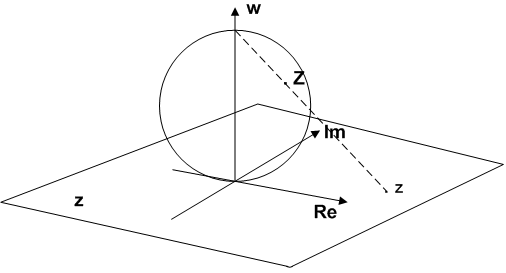
\includegraphics[scale=0.2]{ch1/image1.png}
        \captionof{figure}{Sphère de Riemann}
        \end{wrapfigure}
        Il s'agit d'une sphère de rayon unité qui admet le plan complexe comme plan passant par
        l'équateur de la sphère. On va pouvoir associer tout point du plan complexe à la sphère 
        en traçant une droite reliant le point du plan complexe au pôle de la sphère. Si le point
        est intérieur au plan complexe, le point d'intersection se trouvera à l'hémisphère sud et si ce n'est
        pas le cas, il se trouvera à l'hémisphère nord.\\
        
        Cette visualisation permet d'associer tout point de la sphère à un point du plan complexe, le
        point du pôle étant pour un point situé à l'infini.
        
        
        \subsubsection{Définitions et expressions équivalentes}
        L'expression 
        \begin{equation}
        \lim\limits_{z\rightarrow z_0} f(z) = \infty
        \end{equation}
        est équivalente à 
        \begin{equation}
        \forall \epsilon > 0, \exists \delta > 0\ t.q.\ si\ 0 < |z-z_0| < \delta,\ alors |f(z)| > \frac{1}{\epsilon}
        \end{equation}
        est équivalente à
        \begin{equation}
        Si\ 0\ < |z-z_0| < \delta,\ alors\ |1/f(z) - 0| < \epsilon
        \end{equation}
        d'où
        \begin{equation}
        \lim\limits_{z\rightarrow z_0} f(z) = \infty \Leftrightarrow \lim\limits_{z\rightarrow z_0} \frac{1}{f(z)} = 0
        \end{equation}
        
        En procédant de la même manière, on a, dans le cas où la limite
 		vaut $w_0$ (voir slide 19/28) 
 		\begin{equation}
 		\lim \limits _{z \rightarrow \infty} f(z) = w_0 \Leftrightarrow \lim \limits _{z \rightarrow 0} f(\frac{1}{z}) = w_0 
 		\end{equation}

        
        
    \subsection{Continuité}
    Commençons par une définition intuitive de la continuité. La fonction $f$ est continue
    en $z_0$ si et seulement si :
        \begin{enumerate}
        \item $z_0 \in D$
        \item $\lim\limits_{z\rightarrow z_0} f(z)$ existe
        \item $\lim\limits_{z\rightarrow z_0} f(z) = f(z_0)$
        \end{enumerate}
    De façon plus formelle, cela donne :
    \begin{equation}
    \forall \epsilon > 0, \exists \delta > 0\ t.q.\ si\ |z-z_0| < \delta\ alors\ |f(z) - f(z_0)|\leq \epsilon
    \end{equation}
    Les propriétés qui découlent de cette définition sont identiques à celles définies pour les
    nombres réels.
    
    
    \subsection{Dérivée}
    La définition de la dérivée en un point ($z_0$) n'a (heureusement) pas changé depuis :
    \begin{equation}
    f'(z_0) = \lim\limits_{z\rightarrow z_0} \frac{f(z)-f(z_0)}{z-z_0}
    \end{equation}
    pour autant que cette limite existe. Rappelons que la dérivabilité implique la continuité,
    mais que la réciproque de cette proposition est fausse.\\
    
    \theor{\textsc{Équations de Cauchy-Riemann}\\
    Si $f(z) = u(x,y) +iv(x,y)$ est dérivable en $z_0=x+iy_0$, alors les dérivées partielles
    d'ordre 1 de $u$ et $v$ existent en $(x_0,y_0)$ et
    \begin{equation}
    \frac{\partial u}{\partial x}|_{(x_0,y_0)} = \frac{\partial v}{\partial y}|_{(x_0,y_0)}
    \end{equation}
    et
    \begin{equation}
    \frac{\partial u}{\partial y}|_{(x_0,y_0)} = -\frac{\partial v}{\partial x}|_{(x_0,y_0)}
    \end{equation}
    En outre,
    \begin{equation}
    f'(z_0) = \frac{\partial u}{\partial x}|_{(x_0,y_0)} + i\frac{\partial v}{\partial x}|_{(x_0,y_0)}
    \end{equation}}
    
    
    \begin{proof}
    Par hypothèse, supposons que la dérivée $f'(z_0)$ existe. Notons $\Delta z = \Delta x +i\Delta y$.
    Par le théorème sur les limites, écrivons les expressions en tenant comptes des parties Re et Im.
    \begin{equation}
    \begin{array}{ll}
     Re[f'(z_0)] &=  \lim\limits_{(\Delta x,\Delta y) \rightarrow (0,0)} \text{Re}\left[\frac{f(z_0+\Delta z) - f(z_0)}{\Delta z} \right]\\
     Im[f'(z_0)] &=  \lim\limits_{(\Delta x,\Delta y) \rightarrow (0,0)} \text{Im}\left[\frac{f(z_0+\Delta z) - f(z_0)}{\Delta z} \right]\\
    \end{array}
    \end{equation}
    
    Il faut maintenant écrire l'expression de la dérivée afin d'identifier les parties réelle
    et imaginaire
    \begin{equation}
    \frac{f(z_0+\Delta z)-f(z_0)}{\Delta z} = \frac{u(x_0+\Delta x, y_0 + \Delta y) - u(x_0, y_0)}{\Delta x + i\Delta y}
    + i \frac{v(x_0+\Delta x, y_0 + \Delta y) - v(x_0,y_0)}{\Delta x + i\Delta y}
    \end{equation}
    On remarque que $(\Delta x, \Delta y)$ est quelconque dans un voisinage de (0,0). Considérons
    deux cas particuliers :\\
    
    \textbf{Cas particulier 1 : $(\Delta x, 0) \rightarrow (0,0)$}\\
    Dans ce cas, nous avons :
    \begin{equation}
    \begin{array}{ll}
     Re[f'(z_0)] &= \lim\limits_{\Delta x\rightarrow 0} \frac{u(x_0+\Delta x, y_0) - u(x_0, y_0)}{\Delta x}\\
     Im[f'(z_0)] &= \lim\limits_{\Delta x\rightarrow 0} \frac{v(x_0+\Delta x, y_0) - v(x_0, y_0)}{\Delta x}
    \end{array}
    \end{equation}
    On trouve dès lors, en identifiant la première et deuxième expression respectivement comme la dérivée
    partielle de u (resp. v) par rapport à x :
    \begin{equation}
    f'(z_0) = \frac{\partial u}{\partial x}|_{(x_0,y_0)} + i \frac{\partial v}{\partial x}|_{(x_0,y_0)} 
    \end{equation}
    
    \textbf{Cas particulier 2 : $(0,\Delta y) \rightarrow (0,0)$}\\
    \begin{equation}
    \begin{array}{ll}
     Re[f'(z_0)] &= \lim\limits_{\Delta y\rightarrow 0} \frac{u(x_0, y_0+\Delta y) - u(x_0, y_0)}{\Delta y}\\
     Im[f'(z_0)] &= -\lim\limits_{\Delta y\rightarrow 0} \frac{v(x_0, y_0+\Delta y) - v(x_0, y_0)}{\Delta y}
    \end{array}
    \end{equation}
    On identifie les dérivées partielles des fonctions par rapport à $y$ (le signe négatif dans la seconde
    expression vient de $1/i = -i$. On trouve :
    \begin{equation}
    f'(z_0) = \frac{\partial v}{\partial y}|_{(x_0,y_0)} - i\frac{\partial u}{\partial y}|_{(x_0,y_0)}
    \end{equation}
    
    On trouve dès lors deux expressions pour la même dérivée. Par l'unicité de la limite, ces deux expressions
    sont forcément égales. Leur égalité donne le résultat recherché.
    \end{proof}
    
    \theor{\textsc{Conditions suffisantes d'existence}
    Soit $f(z) = u(x,y) +iv(x,y)$ définie dans un voisinage de $z_0 = x_0 +iy_0$.\\ Si les dérivées partielles
    d'ordre 1 de $u$ et $v$ par rapport à $x$ et $y$
    \begin{enumerate}
    \item existent dans ce voisinage
    \item sont continues en $(x_0,y_0)$
    \item satisfont les équations de Cauchy-Riemann en $(x_0,y_0)$
    \end{enumerate}
    alors $f'(z_0)$ existe.\footnote{Voir livre de référence pour la démonstration.}}
    
    
    \subsection{Fonction analytique}
        \subsubsection{Définition}
    Par définition, une \textit{fonction $f$ est analytique (holomorphe ou régulière) en $z_0$ s'il existe un
    voisinage de $z_0$ tel que $f$ est dérivable en tout point du voisinage.}\\
    \exemple{La fonction $f(z) = 1/z$ est analytique pour $z\neq0$. Par contre la fonction $f(z) = |z|^2$ n'est
    jamais analytique. Par unicité de la limite, celle-ci doit être identique. Or, aucun voisinage de zéro de 
    la fonction n'est dérivable, elle n'est donc analytique nul part.}\ \\
    
    On définira une fonction $f$ \textbf{entière} ssi celle-ci est analytique $\forall z \in \mathbb{C}$.
    
        \subsubsection{Point singulier (!)}
        Le point $z_0$ est singulier de $f$ si $f$  n'est pas analytique en $z_0$, alors que $f$ est analytique
        en certains points de tout voisinage de $z_0$.\\
        \exemple{La fonction $f(z) = |z|^2$ n'a pas de points singuliers. Les points singuliers de $f(z) : P(z)/
        Q(z)$ (tous deux polynômes) : $\{z\in\mathbb{C} : Q(z) = 0$.\}}\ \\
        
        \prop{Si deux fonctions $f_1$ et $f_2$ sont analytiques en $z_0$, leur somme et leur produit sont 
        analytiques en $z_0$; la quotient $f_1/f_2$ est analytique en $z_0$ si $f_2(z_0) \neq 0$.}
        
        
    \subsection{Principe de réflexion}
    \retenir{Considérons une fonction analytique dans un domaine ouvert $D$ contenant un segment de l'axe 
    des $x$, et qui est symétrique par rapport à cet axe. On a : 
    \begin{equation}
    \overline{f(z)} = f(\overline{z})
    \end{equation}
    pour tout $z$ dans $D$ si et seulement si $f(x)$ est réel pour tout point $x$ du segment.}\ \\
    
    \exemple{Faisons deux exemples dont le premier vérifie le principe et pas le second :
    \begin{enumerate}
    \item Soit $f(z) = z+1$. Si j'évalue $f(\overline{z})$ je trouve bien $\overline{z}+1 = \overline{f(z)}$
    \item Soit $f(z) = z+i$. Si j'évalue en $\overline{z}$ je trouve $\overline{z}-1 \neq \overline{f(z)}$
    \end{enumerate}}